\subsection{Umsetzung Graph}
\begin{frame}
\begin{center}
\begin{footnotesize}
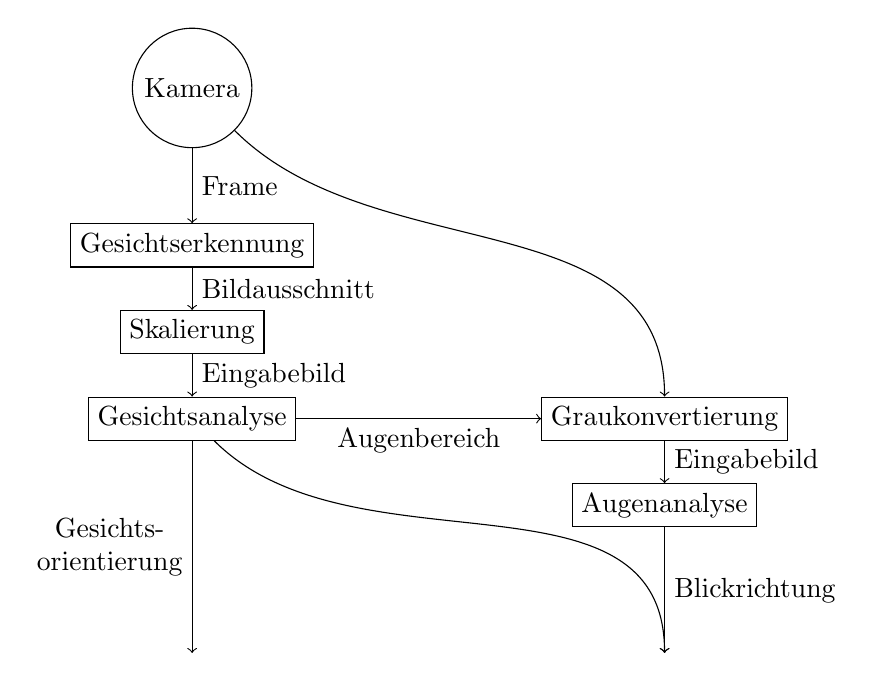
\begin{tikzpicture}
	\node[circle,draw,align=center] (C) at(0,0) {Kamera};
	\node[draw,align=center] (F) at(0,-2)  {Gesichtserkennung};
	\node[draw,align=center] (S) at(0,-3.1)  {Skalierung};
	\node[draw,align=center] (G) at(6,-4.2)  {Graukonvertierung};
	\node[draw,align=center] (A) at(0,-4.2)  {Gesichtsanalyse};
	\node[draw,align=center] (E) at(6,-5.3)  {Augenanalyse};
	
	\node (outA) at(0,-7.3)  {};
	\node (outB) at(6,-7.3)  {};
	
	\draw[->] (E)to node[right,align=center]{Blickrichtung}(outB);
	\draw[->] (A)to[out=-45,in=90] node[right]{}(outB);
	
	\draw[->] (C)to node[right]{Frame}(F);
	\draw[->] (F)to node[right]{Bildausschnitt}(S);
	\draw[->] (S)to node[right]{Eingabebild}(A);
	\draw[->] (A)to node[left,align=center]{Gesichts-\\orientierung}(outA);
	
	\draw[->] (A)to node[below]{Augenbereich}(G);
	\draw[->] (C)to[out=-45,in=90] node[left]{}(G);
	\draw[->] (G)to node[right]{Eingabebild}(E);
\end{tikzpicture}
\end{footnotesize}
\end{center}
\end{frame} % Anstelle von Gliederung
\subsection{Intention}
\begin{frame}
Für die Bestimmung der Blickrichtung hat die Augenregion eine besondere Bedeutung.
\begin{itemize}
	\item<1-> OpenFace verwendet Landmarks für das Augenlid, Iris und Pupille
	\item<1-> Bestimmung der Blickrichtung aus den Landmarks
	\item<1-> ElSe zur Bestimmung der Pupille
\end{itemize}
Verfahre muss stabil bei sehr keinen Bildern arbeiten.
\end{frame}
\begin{frame}
ElSe erwartet ein hochauflösendes Graubild des Auges mit hohem Kontrast zwischen Pupille und Iris.
\begin{figure}
	\centering
	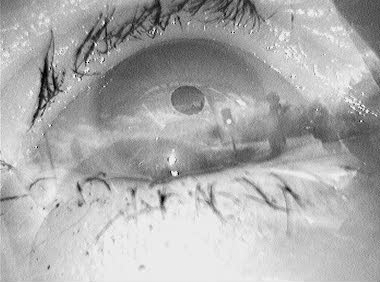
\includegraphics[height=0.3\textheight]{images/Eye_Gray}
	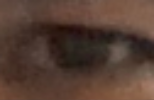
\includegraphics[height=0.3\textheight]{images/Auge_4}
	\label{fig:eyegray}
\end{figure}
Eingabe ist ein niedrig aufgelöstes Farbbild.
\end{frame}
\subsection{Verfahren}
\begin{frame}
\begin{center}
\begin{columns}
	\begin{column}{\linewidth}<1->
		\begin{tabular}{|C{4.2cm}|C{2.03cm}|C{3.5cm}|}
		\hline
		Eingabebid&\tabbild[height=0.1\textheight]{images/Auge}&{\tiny $G_{new} = \dfrac{(G-G_{min})\cdot V_{max}}{G_{max}-G_{min}}$}\\\hline
		Gleam-Verfahren	&\tabbild[height=0.1\textheight]{images/Auge_2Gray}&{\tiny $\dfrac{R^{\frac{1}{2,2}} + G^{\frac{1}{2,2}} + B^{\frac{1}{2,2}}}{3}$}\\\hline
		Gleam-New-Verfahren&\tabbild[height=0.1\textheight]{images/Auge_1Gray}&{\scriptsize $\dfrac{R^{r} + G^{g} + B^{b}}{3},~\frac{\log(V_{\max})}{\log(\{R,G,B\}_{\max})}$}\\\hline
		Luminance-Verfahren&\tabbild[height=0.1\textheight]{images/Auge_0Gray}&{\scriptsize $0,299 R + 0,587 G + 0,114 B$}\\\hline
		Min-Verfahren&\tabbild[height=0.1\textheight]{images/Auge_4Gray}& $\min(R,G,B)$\\\hline
		Max-Verfahren&\tabbild[height=0.1\textheight]{images/Auge_5Gray}& $\max(R,G,B)$\\\hline
		Quadrat-Verfahren&\tabbild[height=0.1\textheight]{images/Auge_3Gray}&{\scriptsize $\dfrac{R^2+G^2+B^2}{3}$}\\\hline
		\end{tabular}
	\end{column}
\end{columns}
\end{center}
\end{frame}